\documentclass[a4paper,11pt]{article} %indique la classe du document, et les options

%le pr\'eambule
\usepackage[english]{babel}
\usepackage{graphicx}
\usepackage{array}
\usepackage{multicol}
\usepackage{fancyhdr}
\usepackage{listings}
\setlength{\headheight}{15.2pt}
\pagestyle{fancy}
\selectlanguage{english}


%Titre
\makeatletter
\def\maketitle{

	\begin{multicols}{2}
		{\begin{center}
		{\LARGE \@title}\\
		\rule{3cm}{1pt}
	\end{center}}
		\begin{flushright}
			{\includegraphics[width=0.5\linewidth]{../../Newcastle-University.jpg}}\\
			{\@date}\\
		\end{flushright}
	\end{multicols}	
	\vspace{1cm}
}
\def\email#1{\def\@email{#1}}
\makeatother
\email{nicolas.desfeux@gmail.com}
\date{\today}
\author{Nicolas Desfeux}
\title{
{Coursework 2
}}

\renewcommand{\thesection}{\textnormal{\roman{section}})} 
\renewcommand{\thesubsection}{~~\textnormal{\alph{subsection}})} 
%document principal 

\begin{document}
\maketitle
\lhead{Nicolas Desfeux}
\rhead{Student No :110477367 - Erasmus student}

\section{Argue on the system design}
Here is a vue of the actual system : \\
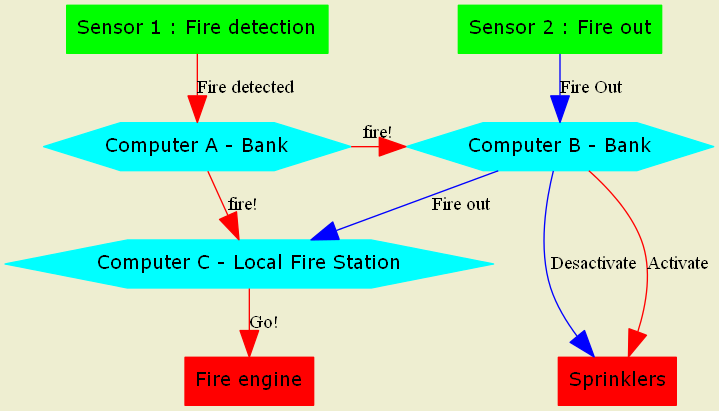
\includegraphics[width=1.2\linewidth]{ex2.png}
Waiting for (2d+e) time units after a "fire!" message have been received looks like a good idea, as it correspond to : 
\begin{itemize}
\item d : Max time for A to send message to B
\item d : Max time for B to send message to C
\item e : Max time that can elapsed between sprinklers on and the sensors informing B that fire has been put out.
\end{itemize}
\subsection{Fire engines send for nothing}
We're looking here for a situation where a "fire out" is not send on time to the local fire station.
Let's assume that two fire start : 
\begin{enumerate}
\item The first fire start. Message "fire!" is sent from A to B.(time 0)
\item Before B receive the message, a second fire start.(time a, between 0 and d)
\item B receive the fire message, and start the sprinkler.
\item First fire is off. second is still on , so A is still sending message to C. B don't send fire out, as the second fire is still on.
\item C is now receiving message for more 2d+e, so send fire engines.
\item Second fire is off, thanks to sprinklers. 
\item B send fire out message, and the time could be between 2d+e and (2d+e) +a.
\item As fire engines are here, no more fire.
\end{enumerate}
There is clearly a system trouble here.
\subsection{Fire engines not send as fire is on}
We are looking here for the cases where fire engine are not sent as they should be.
It could happens in this case : 
\begin{enumerate}
\item First fire start, time 0.
\item A send message to B and C. B starts the sprinklers.
\item Sprinklers are on, and achieve to kill the first fire.
\item B send to C a "fire out!"
\item Before C receive the message, a second fire start (a units time before C receive the message).
\item A send message "fire!"to B and C. 
\item C receive b message, reboot counter. Then receive message from A.
\item Sprinklers can't kill the second fire.
\item C sent fire engines, but it could 2d+e+a that the fire started.
Here fire engines are send in a good purpose, but at the wrong timing. The same problem happens when two fire start, and the second one is kill by the sprinkler before fire engine are send for the first one.
\end{enumerate}
\newpage
\section{Producing a correct system}
\paragraph{}We now assume that A and B use logical clocks, and they use those clocks to timestamp their messages. Those clocks increase on each local actions they execute. We also decide that A and B will have the same increment value.\\
We'll keep the same system architecture, we'll modify A, B and C actions and reactions to messages.
Computer A still receive informations from fire detection sensors. each sensors notification increase the A clock value. A raise two events : sending message to B (timestamp x), and sending message to C (timestamp x+i, i the increment of A clock).
\\Computer B have set his logical clock to the value of the timestamp (let's call it x for the example) received from the "fire!" message from A. If fire put out detection sensors warn B before B receive a new fire message from A : B clocks increment, then B send a message with timestamp x + i, with i the increment of the B clock, to computer C, and then start the sprinkler. Otherwise, it timestamp is updated to the new one send by A.
\\Computer C receive messages from A : it counter move until reach 2d+e, then send the fire engines. If a message is received from B, C will compare the two messages he received : the last received from A, and the last from B.
\\If timestamp from B is lower or equal to timestamp from A, C have to keep is counter value. If timestamp from B is higher than timestamp from A, then C reset his counter. AS soon as C counter reach the critical value, fire engines are send.
\\By using logical for A and B, we can solve problems describe in the previous part.

\section{Condition for correctness with physical clocks}
The conditions needed for the system we design before are the folllowing :
\begin{itemize}
\item The time between the A sending message to B and A sending message to C must be the same as B getting info from sensors and sending message to C (message from A to C have to be delayed).
\item The condition for C must change :  If timestamp from B is lower or equal to timestamp+ epsilon from A, C have to keep is counter value. If timestamp from B is higher than timestamp+epsilon from A, then C reset his counter. As soon as C counter reach the critical value, fire engines are send.
\end{itemize}
\end{document}